\documentclass[english, fontsize=12pt, paper=a4, twoside=false, draft=true, pagesize=auto, version=last, DIV=16]{scrartcl}


\let\counterwithout\relax
\let\counterwithin\relax

\usepackage[utf8]{inputenc}
%Für Tabellen
\usepackage{tabularx}

% Für Absätze in Bildbeschreibung
\usepackage{caption}

% Zur nummerierten Aufzählung, mit automatischem Einrücken
\usepackage{paralist}
\usepackage{enumitem}
\usepackage{csquotes}


% mitwachsender Implikationspfeil mit Text
\makeatletter
\newcommand{\xRightarrow}[2][]{\ext@arrow 0359\Rightarrowfill@{#1}{#2}}
\makeatother


% Java Code Einbinden
\usepackage{listings}
\usepackage{color}
\usepackage[svgnames]{xcolor}



% Um einzelne Seiten zu drehen
\usepackage{pdflscape}
%\usepackage{rotating}
%\usepackage{lscape}


\usepackage{lmodern}
\usepackage[T1]{fontenc}
%\usepackage[latin1]{inputenc}
\usepackage{babel}
\usepackage[utf8]{inputenc}
\usepackage{stmaryrd}
\usepackage{extarrows}
\usepackage{ulem}



%Zur Bildnummerierung
\usepackage{chngcntr}
\usepackage{mathtools}
\usepackage{amsmath}
%Zur Verwendung von "chngcntr": \counterwithin{figure}{section}


%Euro-Zeichen
\usepackage{eurosym}

\usepackage{float}

\usepackage{amsmath}
\usepackage{acronym} %[''Optionen'']
\usepackage{esvect}  %Für Vektorpfeile, Aufruf mit \vv{Vektorname}

% Für schön Buchstaben1
\usepackage{mathrsfs}
\usepackage{suetterl}
\usepackage{calligra}

% Einzelne Seite drehen
\usepackage{lscape}


% ----------------------------------------------------------------------------------------
% ----------------------------------- Beginn Code einbinden ------------------------------
% ----------------------------------------------------------------------------------------
% Default fixed font does not support bold face
\DeclareFixedFont{\ttb}{T1}{txtt}{bx}{n}{12} % for bold
\DeclareFixedFont{\ttm}{T1}{txtt}{m}{n}{12}  % for normal

% Custom colors
\usepackage{color}
\definecolor{deepblue}{rgb}{0,0,0.5}
\definecolor{deepred}{rgb}{0.6,0,0}
\definecolor{deepgreen}{rgb}{0,0.5,0}

\usepackage{listings}

% Python style for highlighting
\newcommand\pythonstyle{\lstset{
language=Python,
basicstyle=\fontsize{10}{10}\selectfont\ttfamily,  % oder \ttm,
otherkeywords={self},             % Add keywords here
keywordstyle=\ttb\color{deepblue},
emph={MyClass,__init__},          % Custom highlighting
emphstyle=\ttb\color{deepred},    % Custom highlighting style
stringstyle=\color{deepgreen},
frame=tb,                         % Any extra options here
showstringspaces=false            %
}}


% Python environment
\lstnewenvironment{python}[1][]
{
\pythonstyle
\lstset{#1}
}
{}

% Python for external files
\newcommand\pythonexternal[2][]{{
\pythonstyle
\lstinputlisting[#1]{#2}}}


% ----------------------------------------------------------------------------------------
% ------------------------------------ Ende Code einbinden -------------------------------
% ----------------------------------------------------------------------------------------



%%% Neue Kommandos/Begriffe %%%
%\renewcommand{\thesection}{\arabic{section}}
% Für Fußnoten ohne Nummer
%\renewcommand{\thefootnote}{}



% Für die Normalschrift im Abkürzungsverzeichnis, das Paket "acronym" veranlasst eine andere Schriftart bei Abkürzungen.
\newcommand{\Rule}{\rule{\textwidth}{0.5mm}}
% \newcommand{\absatzParagraph}[1]{\paragraph{#1}\mbox{}\\}


\usepackage{geometry}
\newgeometry{left=18mm,right=18mm,top=15mm,bottom=15mm}
\footskip = 22pt

\usepackage{setspace}  % Paket einbinden
\onehalfspacing        % einstellen des Zeilenabstandes auf 1,5
\setlength{\parindent}{0in}
\usepackage{amsmath}
\usepackage[amsmath,amsthm,thmmarks]{ntheorem}
\usepackage{amssymb}


% Komplexitätsklassen
% \usepackage[bold,full]{complexity}


% Für Pseudocode
\usepackage{algorithm}
\usepackage{algpseudocode}


% für mehrzeilige Kommentare
\usepackage{verbatim}


% ------------- Beginn Definition von: Satz, Lemma Definition usw. -------------
\theoremstyle{break}
%\theoremstyle{definition}
\theorembodyfont{\upshape}
\newtheorem{defin}{Definition}[section] % Präambel
\newtheorem{lemma}[defin]{Lemma}
\newtheorem{satz}[defin]{Satz}
\newtheorem{kor}[defin]{Korollar}
\newtheorem{beo}[defin]{Beobachtung}
\newtheorem{bemerk}[defin]{Bemerkung}
\newtheorem{übung}[defin]{Übung}

%  ------------- Ende Definition von: Satz, Lemma Definition usw. -------------

% Für URLs
\usepackage{url}
\usepackage{hyperref}
\hypersetup{final}



\usepackage{animate}
\usepackage{graphicx}
\usepackage{graphics}
\usepackage{hyphenat}


\usepackage{tikz}
\usepackage{tkz-euclide}
\usetikzlibrary{arrows, matrix, shapes, decorations.pathmorphing,calc,patterns,through,intersections}

\newcommand*\bigO{\mathcal{O}}



\begin{document}


\title{
\vspace*{-10mm}
Exercise 4 \\[-3pt]
{\Large $\mathrm{for \ the \ lecture}$} \\[-3pt]
{\LARGE \textbf{Computational Geometry}}
}
\author{Dominik Bendle, Stefan Fritsch, Marcel Rogge and Matthias Tschöpe}
\maketitle
\vspace*{-10mm}

\section*{\large Exercise 1 (Image Compression using Quadtrees) {\normalsize \hfill (1 + 3 + 1 + 1 points)}}
\textbf{a)} \par
\underline{Best Case:} The data are clustered in the same region/subtree.
$\Rightarrow$ The tree is filled up subtree by subtree. \par
Example for the worst case (image filled up with 25 \% of data points): \par
\vspace*{-7mm}
\begin{minipage}[t]{0.48\textwidth}
\begin{figure}[H]
\centering
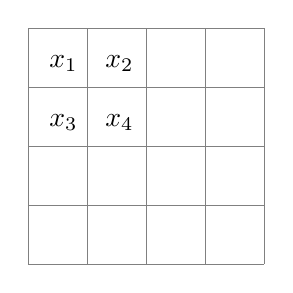
\begin{tikzpicture}[>=latex, thick, inner sep=0pt, scale=0.75]
	\node[](x1) at (0.6,3.4) {$x_1$};
	\node[](x2) at (1.55,3.4) {$x_2$};
	\node[](x3) at (0.6,2.4) {$x_3$};
	\node[](x4) at (1.55,2.4) {$x_4$};

	\draw[step=1cm,gray,very thin] (0,0) grid (4,4);		
\end{tikzpicture}
\label{Result after step 1}
\end{figure} \par
\end{minipage} \hspace*{5mm}
\begin{minipage}[t]{0.45\textwidth}
	\begin{figure}[H]
		\centering
		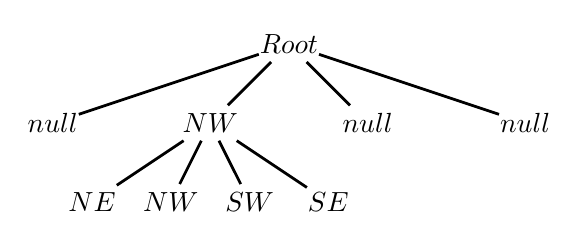
\begin{tikzpicture}[>=latex, thick, inner sep=0pt, scale=0.5]
			\node[minimum size=12pt] (root) at (0,0) {$Root$};
			
			\node[minimum size=12pt] (null1) at (-6,-2) {$null$};
			\node[minimum size=12pt] (nw) at (-2,-2) {$NW$};
			\node[minimum size=12pt] (null2) at (2,-2) {$null$};
			\node[minimum size=12pt] (null3) at (6,-2) {$null$};
			
			\node[minimum size=12pt] (ne_c) at (-5,-4) {$NE$};			
			\node[minimum size=12pt] (nw_c) at (-3,-4) {$NW$};			
			\node[minimum size=12pt] (sw_c) at (-1,-4) {$SW$};			
			\node[minimum size=12pt] (se_c) at (1,-4) {$SE$};			
			
			\draw[-, line width=1pt](root) edge (null1);
			\draw[-, line width=1pt](root) edge (nw);
			\draw[-, line width=1pt](root) edge (null2);
			\draw[-, line width=1pt](root) edge (null3);
			
			\draw[-, line width=1pt](nw) edge (ne_c);
			\draw[-, line width=1pt](nw) edge (nw_c);
			\draw[-, line width=1pt](nw) edge (sw_c);
			\draw[-, line width=1pt](nw) edge (se_c);
		\end{tikzpicture}
	\label{Result after step 1 tree}
	\end{figure} \par
\end{minipage} \par
\vspace*{10mm}
\underline{Worst Case:} The data points are distributed all over the image and not clustered. $\Rightarrow\ $ The data are distributed evenly among the subtrees. \par
Example for the worst case (image filled up with 25 \% of data points):
\begin{figure}[H]
\centering
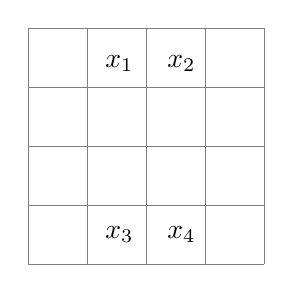
\begin{tikzpicture}[>=latex, thick, inner sep=0pt, scale=0.75]
	\node[](x1) at (1.55,3.4) {$x_1$};
	\node[](x2) at (2.6,3.4) {$x_2$};
	\node[](x3) at (1.55,0.5) {$x_3$};
	\node[](x4) at (2.6,0.5) {$x_4$};

	\draw[step=1cm,gray,very thin] (0,0) grid (4,4);		
\end{tikzpicture} \par
\vspace*{5mm}
\label{Result after step 1}
\end{figure} \par
	\begin{figure}[H]
		\centering
		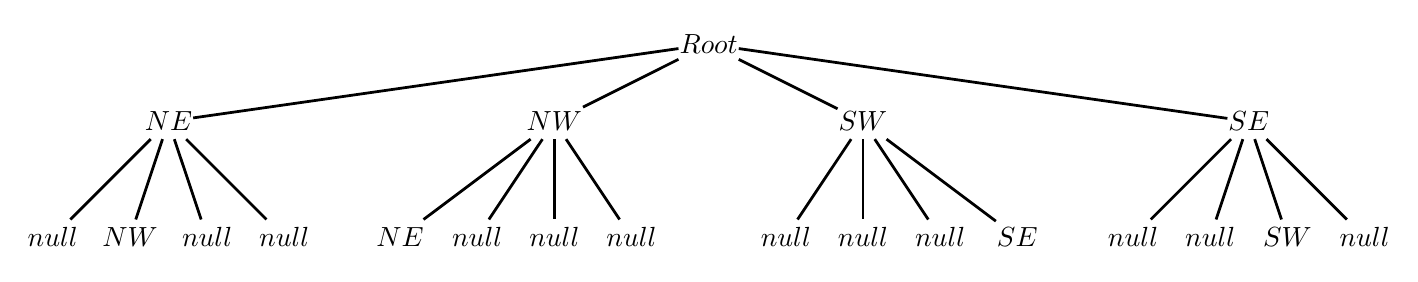
\begin{tikzpicture}[>=latex, thick, inner sep=0pt, scale=0.49]
			\node[minimum size=12pt] (root) at (0,0) {$Root$};
			
			\node[minimum size=12pt] (ne) at (-14,-2) {$NE$};
			\node[minimum size=12pt] (nw) at (-4,-2) {$NW$};
			\node[minimum size=12pt] (sw) at (4,-2) {$SW$};
			\node[minimum size=12pt] (se) at (14,-2) {$SE$};
			
			\node[minimum size=12pt] (ne_c1) at (-17,-5) {$null$};			
			\node[minimum size=12pt] (nw_c1) at (-15,-5) {$NW$};			
			\node[minimum size=12pt] (sw_c1) at (-13,-5) {$null$};			
			\node[minimum size=12pt] (se_c1) at (-11,-5) {$null$};			
			
			\node[minimum size=12pt] (ne_c2) at (-8,-5) {$NE$};			
			\node[minimum size=12pt] (nw_c2) at (-6,-5) {$null$};			
			\node[minimum size=12pt] (sw_c2) at (-4,-5) {$null$};			
			\node[minimum size=12pt] (se_c2) at (-2,-5) {$null$};
			
			\node[minimum size=12pt] (ne_c3) at (2,-5) {$null$};			
			\node[minimum size=12pt] (nw_c3) at (4,-5) {$null$};			
			\node[minimum size=12pt] (sw_c3) at (6,-5) {$null$};			
			\node[minimum size=12pt] (se_c3) at (8,-5) {$SE$};
			
			\node[minimum size=12pt] (ne_c4) at (11,-5) {$null$};			
			\node[minimum size=12pt] (nw_c4) at (13,-5) {$null$};			
			\node[minimum size=12pt] (sw_c4) at (15,-5) {$SW$};			
			\node[minimum size=12pt] (se_c4) at (17,-5) {$null$};
			
			\draw[-, line width=1pt](root) edge (ne);
			\draw[-, line width=1pt](root) edge (nw);
			\draw[-, line width=1pt](root) edge (sw);
			\draw[-, line width=1pt](root) edge (se);
			
			\draw[-, line width=1pt](ne) edge (ne_c1);
			\draw[-, line width=1pt](ne) edge (nw_c1);
			\draw[-, line width=1pt](ne) edge (sw_c1);
			\draw[-, line width=1pt](ne) edge (se_c1);
			
			\draw[-, line width=1pt](nw) edge (ne_c2);
			\draw[-, line width=1pt](nw) edge (nw_c2);
			\draw[-, line width=1pt](nw) edge (sw_c2);
			\draw[-, line width=1pt](nw) edge (se_c2);
			
			\draw[-, line width=1pt](sw) edge (ne_c3);
			\draw[-, line width=1pt](sw) edge (nw_c3);
			\draw[-, line width=1pt](sw) edge (sw_c3);
			\draw[-, line width=1pt](sw) edge (se_c3);
			
			\draw[-, line width=1pt](se) edge (ne_c4);
			\draw[-, line width=1pt](se) edge (nw_c4);
			\draw[-, line width=1pt](se) edge (sw_c4);
			\draw[-, line width=1pt](se) edge (se_c4);
		\end{tikzpicture}
	\label{Result after step 1 tree}
\end{figure} \par
\newpage


\textbf{b)} \par
We assume in Worst Case that our squared input image is filled up with at least 25 \% of data points. So our tree is a complete $4-$regular tree. Since, $e$ is the edge length of the squared image, the depth of our Quad-Tree in the Worst Case is given by $log_4(e^2) = 2 \cdot log_4(e)$. Now, we can compute the number of inner vertices as: \par
\vspace*{-3mm}
\begin{equation}
\begin{aligned}
\sum\limits_{\ell = 0}^{log_4(e^2) - 1} 4^\ell
\end{aligned}
\end{equation}
Further, we know the number of leafs is: \par
\vspace*{-3mm}
\begin{equation}
\begin{aligned}
4^{log_4(e^2)}
\end{aligned}
\end{equation} \par
Since, each inner vertex has 5 Pointer (four to his children and one to its parent vertex) except the root node (the root node does not have a parent, therefore at the end $-8 \text{ Byte}$) and each pointer needs 8 Byte, so we need: \par
\vspace*{-3mm}
\begin{equation}
\begin{aligned}
\left( \sum\limits_{\ell = 0}^{log_4(e^2) - 1} 4^\ell \right) \cdot 5 \cdot 8 \text{ Byte} - 8 \text{ Byte}= \frac{1}{3}\left( e^2 - 1 \right) \cdot 5 \cdot 8 \text{ Byte} - 8 \text{ Byte}
\end{aligned}
\end{equation} \par
For the leaf nodes we need: \par
\vspace*{-3mm}
\begin{equation}
\begin{aligned}
x \cdot 4^{log_4(e^2)} \cdot 8 \text{ Byte} = x \cdot e^2 \cdot 8 \text{ Byte}
\end{aligned}
\end{equation} \par
storage, where $x$ is as given the ration of non-zero data. The leads to the following algorithm: \par

\begin{algorithm}
\caption{Calculate $\frac{s_{new}}{s_{old}}$ ratio}
\label{Alg f} \par
\medskip
{f($e, x$)} \par
\vspace*{-3mm}
\begin{itemize}[leftmargin=20mm]
\item[\textbf{Input:}] edge length $e$ and fraction of non-zero data $x$. \\[-20pt]
\item[\textbf{Ouput:}] ratio $\frac{s_{new}}{s_{old}}$.
\end{itemize} \par
\vspace*{-3mm}
\begin{algorithmic}[1]
	\State $s_{old} \coloneqq e^2 \cdot 8$Byte
	\State \texttt{size\_not\_null\_data} $\coloneqq x \cdot s_{old}$
	\State \texttt{tree\_size} $\coloneqq \left(\frac{1}{3}\left( e^2 - 1 \right) \cdot 5 + x \cdot e^2 \right) \cdot 8 \text{ Byte} - 8 \text{ Byte}$
	\State $s_{new} \coloneqq \texttt{size\_not\_null\_data} + \texttt{tree\_size}$ 
   	\State \Return $\frac{s_{new}}{s_{old}}$
\end{algorithmic}
\end{algorithm}\par
\vspace*{15mm}


\textbf{c)}
First we explain the idea of the function $g$, which computes the storage for the best case. As above, each inner vertex has 5 Pointer (except the root node) and each pointer needs $8 \text{ Byte}$. Similar to the Worst Case, the tree has a maximal depth of $log_4(e^2)$. So, the last inner vertex is on level $log_4(e^2) - 1$. The number of used non-zero data is again $x \cdot e^2$. Hence, we get the following best case function: \par
\newpage
\begin{algorithm}
\caption{Calculate $\frac{s_{new}}{s_{old}}$ ratio}
\label{Alg f} \par
\medskip
{g($e, x$)} \par
\vspace*{-3mm}
\begin{itemize}[leftmargin=20mm]
\item[\textbf{Input:}] edge length $e$ and fraction of non-zero data $x$. \\[-20pt]
\item[\textbf{Ouput:}] ratio $\frac{s_{new}}{s_{old}}$.
\end{itemize} \par
\vspace*{-3mm}
\begin{algorithmic}[1]
	\State $s_{old} \coloneqq e^2 \cdot 8$Byte
	\State \texttt{size\_not\_null\_data} $\coloneqq x \cdot s_{old}$
	\State \texttt{tree\_size} $\coloneqq \left( (log_4(e^2) - 1) \cdot 5 + x \cdot e^2 \right) \cdot 8 \text{ Byte} - 8 \text{ Byte}$
	\State $s_{new} \coloneqq \texttt{size\_not\_null\_data} + \texttt{tree\_size}$ 
   	\State \Return $\frac{s_{new}}{s_{old}}$
\end{algorithmic}
\end{algorithm}\par
\vspace*{5mm}

\underline{Worst Case calculation:} \par
\vspace*{-3mm}
\begin{algorithm}
{f($e=4, x=0.25$)} \par
\begin{algorithmic}[1]
	\State $s_{old} \coloneqq 4^2 \cdot 8$Byte = $128$ Byte
	\State \texttt{size\_not\_null\_data} $\coloneqq 0.25 \cdot s_{old} = 32$ Byte
	\State \texttt{tree\_size} $\coloneqq \left(\frac{1}{3}\left( 4^2 - 1 \right) \cdot 5 + x \cdot e^2 \right) \cdot 8 \text{ Byte} - 8 \text{ Byte} = (25 + 4) \cdot 8 \text{ Byte} - 8 \text{ Byte} = 224$ Byte
	\State $s_{new} 32 + 224 = 256$ 
   	\State \Return $\frac{s_{new}}{s_{old}} = \frac{256}{128} = 2$
\end{algorithmic}
\end{algorithm}\par
\vspace*{3mm}

\underline{Best Case calculation:} \par
\vspace*{-3mm}
\begin{algorithm}
{g($e, x$)} \par
\begin{algorithmic}[1]
	\State $s_{old} \coloneqq 4^2 \cdot 8$Byte = $128$ Byte
	\State \texttt{size\_not\_null\_data} $\coloneqq 0.25 \cdot s_{old} = 32$ Byte
	\State \texttt{tree\_size} $\coloneqq \left( (log_4(4^2) - 1) \cdot 5 + 0.25 \cdot 4^2 \right) \cdot 8 \text{ Byte} - 8 \text{ Byte} = 64 \text{ Byte}$
	\State $s_{new} 32 + 64= 96$ 
   	\State \Return $\frac{s_{new}}{s_{old}} = \frac{96}{128} = 0.75$
\end{algorithmic}
\end{algorithm}\par
\vspace*{15mm}


\textbf{d)}
We have four approaches how we could save even more memory:

1) We assume, each string needs 8 Byte. Instead of using the strings "NE", "SE", "SW" and "NW", we can use integer values. Since, we only need four values, the standard int32 which can store $2^{32}-1$ values is enough. If we assume a boolean value need exact one Bit, then we can do better. We could use two boolean values (2 Bit) which decode the values $1,2,3$ and $4$ as binary value. \par
2) We can eliminate the pointers which point to the data points by saving the data points directly in the tree. \par
3) We skip the rule that every node has to have exactly four child nodes to reduce the memory for storing null-pointers. We can achieve this by saving the leafs of a parent node $p_i$ in a list. This list only contains real data points and no null values. \par
4) Further, for the non-zero-entries, we could try to find duplicates and store them only once. \par
\newpage




\section*{\large Exercise 2 (kD-tree Construction) {\normalsize \hfill (2 points)}}
\vspace*{10mm}
We use two lists $x_{sorted}$ and $y_{sorted}$ and sort them in the $x$ respectively the $y$ direction: \par
\begin{equation}
\begin{aligned}
y_{sorted} & \coloneqq [A,B,C,D,E,F,G,H,I,J,K,L,M] \\[3pt]
x_{sorted} & \coloneqq [M,E,I,H,A,K,D,F,L,B,C,J,G]
\end{aligned}
\end{equation}
Both list have a length of $len(y_{sorted}) = len(y_{sorted}) = 6$. We shorten the given rules by $Ri$, where $i \in \{1,2,3,4\}$. \par
\vspace*{15mm}

\underline{Step 1.} \par
By $R2$ we first have to split in $y-$direction. This means we have to calculate the middle element of the $y_{sorted}$ list, which is $G$. Hence, $G$ is the first vertex in the $kD-$tree. This yields to the following results: \par
\vspace*{-5mm}
\begin{minipage}[t]{0.48\textwidth}
\begin{figure}[H]
\centering
\begin{tikzpicture}[>=latex, thick, inner sep=0pt, scale=0.5]
	
	
	\draw[black,thick,dashed] (0,0) -- (16.6,0) -- (16.6,-11.8) -- (0,-11.8) -- (0,0);
	
	\node[circle, fill, draw=black, minimum size=2pt](a) at (5.92,-0.35) {};
	\node[circle, fill, draw=black, minimum size=2pt](b) at (13.64,-0.69) {};
	\node[circle, fill, draw=black, minimum size=2pt](c) at (14.26,-1.12) {};
	\node[circle, fill, draw=black, minimum size=2pt](d) at (11.07,-1.73) {};
	\node[circle, fill, draw=black, minimum size=2pt](e) at (2.08,-2.75) {};
	\node[circle, fill, draw=black, minimum size=2pt](f) at (12.38,-3.42) {};
	\node[circle, fill, draw=black, minimum size=2pt](g) at (15.67,-4.08) {};
	\node[circle, fill, draw=black, minimum size=2pt](h) at (4.77,-5.32) {};
	\node[circle, fill, draw=black, minimum size=2pt](i) at (3.48,-6.33) {};
	\node[circle, fill, draw=black, minimum size=2pt](j) at (14.75,-8.16) {};
	\node[circle, fill, draw=black, minimum size=2pt](k) at (8.05,-9.56) {};
	\node[circle, fill, draw=black, minimum size=2pt](l) at (12.56,-10.3) {};
	\node[circle, fill, draw=black, minimum size=2pt](m) at (0.67,-11.2) {};
		
		
	\node[](A) at (6.22,-0.6) {$A$};
	\node[](B) at (13.28,-0.9) {$B$};
	\node[](C) at (14.56,-1.42) {$C$};
	\node[](D) at (11.37,-2.03) {$D$};
	\node[](E) at (2.38,-3.05) {$E$};
	\node[](F) at (12.68,-3.72) {$F$};
	\node[](G) at (15.97,-4.38) {$G$};
	\node[](H) at (5.07,-5.62) {$H$};
	\node[](I) at (3.78,-6.63) {$I$};
	\node[](J) at (15.05,-8.46) {$J$};
	\node[](K) at (8.35,-9.86) {$K$};
	\node[](L) at (12.86,-10.6) {$L$};
	\node[](M) at (1.1,-11.5) {$M$};

	\node[](a_start) at (5.92,0) {};
	\node[](a_ende) at (5.92,-1.73) {};
	
	\node[](b_start) at (13.64,0) {};
	\node[](b_ende) at (13.64,-1.12) {};

	\node[](c_start) at (12.38,-1.12) {};
	\node[](c_ende) at (16.6,-1.12) {};
	
	\node[](d_start) at (0.0,-1.73) {};
	\node[](d_ende) at (12.38,-1.73) {};
	
	\node[](e_start) at (2.08,-1.73) {};
	\node[](e_ende) at (2.08,-4.08) {};
	
	\node[](f_start) at (12.38,0) {};
	\node[](f_ende) at (12.38,-4.08) {};
	
	\node[](g_start) at (0.0,-4.08) {};
	\node[](g_ende) at (16.6,-4.08) {};
	
	\node[](h_start) at (4.77,-4.08) {};
	\node[](h_ende) at (4.77,-6.33) {};
	
	\node[](i_start) at (0.0,-6.33) {};
	\node[](i_ende) at (8.05,-6.33) {};
	
	\node[](j_start) at (14.75,-4.08) {};
	\node[](j_ende) at (14.75,-10.3) {};
	
	\node[](k_start) at (8.05,-4.08) {};
	\node[](k_ende) at (8.05,-11.8) {};

	\node[](l_start) at (8.05,-10.3) {};
	\node[](l_ende) at (16.6,-10.3) {};

	\node[](m_start) at (0.67,-6.33) {};
	\node[](m_ende) at (0.67,-11.8) {};
	

	% horizontale Linen	
	\draw[-, line width=1pt](g_start) edge (g_ende);			
\end{tikzpicture}
\label{Result after step 1}
\end{figure} \par
\end{minipage} \hspace*{5mm}
\begin{minipage}[t]{0.45\textwidth}
	\begin{figure}[H]
		\centering
		
\begin{tikzpicture}[>=latex, thick, inner sep=0pt, scale=0.5]
			\node[circle, draw=black, minimum size=15pt](G) at (0,0) {$G$};
		\end{tikzpicture}
	\label{Result after step 1 tree}
	\end{figure} \par
\end{minipage} \par
\vspace*{15mm}



\underline{Step 2.} \par
Now we have to split in $x-$direction. Therefore, we take the $x_{sorted}$ list and split them in two new lists $x_{above}$ and $x_{below}$, where both list are sorted in $x-$direction: \par
\vspace*{-3mm}
\begin{equation}
\begin{aligned}
x_{above} & \coloneqq [E,A,D,F,B,C] \\[3pt]
x_{below} & \coloneqq [M,I,H,K,J,G]
\end{aligned}
\end{equation}
Since, both lists have even length, we have to use $R4$ to calculate the middle elements: \par\vspace*{-3mm}
\begin{equation}
\begin{aligned}
n \coloneqq len(x_{above}) = 6 \ \Longrightarrow \ \text{middle element is } F \\[3pt]
n \coloneqq len(x_{below}) = 6 \ \Longrightarrow \ \text{middle element is } K
\end{aligned}
\end{equation}
By $R3$, we have to order the points above, as the left child and the points below as the right child. This gives us: \newpage


\vspace*{-5mm}
\begin{minipage}[t]{0.48\textwidth}
\begin{figure}[H]
\centering
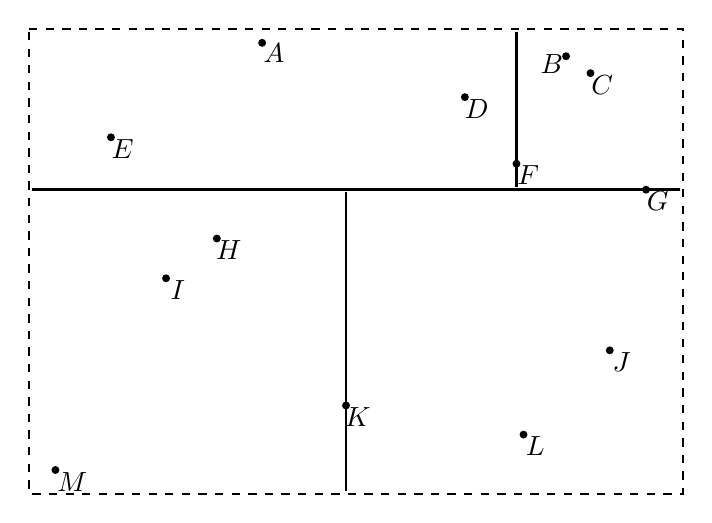
\begin{tikzpicture}[>=latex, thick, inner sep=0pt, scale=0.5]
	
	
	\draw[black,thick,dashed] (0,0) -- (16.6,0) -- (16.6,-11.8) -- (0,-11.8) -- (0,0);
	
	\node[circle, fill, draw=black, minimum size=2pt](a) at (5.92,-0.35) {};
	\node[circle, fill, draw=black, minimum size=2pt](b) at (13.64,-0.69) {};
	\node[circle, fill, draw=black, minimum size=2pt](c) at (14.26,-1.12) {};
	\node[circle, fill, draw=black, minimum size=2pt](d) at (11.07,-1.73) {};
	\node[circle, fill, draw=black, minimum size=2pt](e) at (2.08,-2.75) {};
	\node[circle, fill, draw=black, minimum size=2pt](f) at (12.38,-3.42) {};
	\node[circle, fill, draw=black, minimum size=2pt](g) at (15.67,-4.08) {};
	\node[circle, fill, draw=black, minimum size=2pt](h) at (4.77,-5.32) {};
	\node[circle, fill, draw=black, minimum size=2pt](i) at (3.48,-6.33) {};
	\node[circle, fill, draw=black, minimum size=2pt](j) at (14.75,-8.16) {};
	\node[circle, fill, draw=black, minimum size=2pt](k) at (8.05,-9.56) {};
	\node[circle, fill, draw=black, minimum size=2pt](l) at (12.56,-10.3) {};
	\node[circle, fill, draw=black, minimum size=2pt](m) at (0.67,-11.2) {};
		
		
	\node[](A) at (6.22,-0.6) {$A$};
	\node[](B) at (13.28,-0.9) {$B$};
	\node[](C) at (14.56,-1.42) {$C$};
	\node[](D) at (11.37,-2.03) {$D$};
	\node[](E) at (2.38,-3.05) {$E$};
	\node[](F) at (12.68,-3.72) {$F$};
	\node[](G) at (15.97,-4.38) {$G$};
	\node[](H) at (5.07,-5.62) {$H$};
	\node[](I) at (3.78,-6.63) {$I$};
	\node[](J) at (15.05,-8.46) {$J$};
	\node[](K) at (8.35,-9.86) {$K$};
	\node[](L) at (12.86,-10.6) {$L$};
	\node[](M) at (1.1,-11.5) {$M$};

	\node[](a_start) at (5.92,0) {};
	\node[](a_ende) at (5.92,-1.73) {};
	
	\node[](b_start) at (13.64,0) {};
	\node[](b_ende) at (13.64,-1.12) {};

	\node[](c_start) at (12.38,-1.12) {};
	\node[](c_ende) at (16.6,-1.12) {};
	
	\node[](d_start) at (0.0,-1.73) {};
	\node[](d_ende) at (12.38,-1.73) {};
	
	\node[](e_start) at (2.08,-1.73) {};
	\node[](e_ende) at (2.08,-4.08) {};
	
	\node[](f_start) at (12.38,0) {};
	\node[](f_ende) at (12.38,-4.08) {};
	
	\node[](g_start) at (0.0,-4.08) {};
	\node[](g_ende) at (16.6,-4.08) {};
	
	\node[](h_start) at (4.77,-4.08) {};
	\node[](h_ende) at (4.77,-6.33) {};
	
	\node[](i_start) at (0.0,-6.33) {};
	\node[](i_ende) at (8.05,-6.33) {};
	
	\node[](j_start) at (14.75,-4.08) {};
	\node[](j_ende) at (14.75,-10.3) {};
	
	\node[](k_start) at (8.05,-4.08) {};
	\node[](k_ende) at (8.05,-11.8) {};

	\node[](l_start) at (8.05,-10.3) {};
	\node[](l_ende) at (16.6,-10.3) {};

	\node[](m_start) at (0.67,-6.33) {};
	\node[](m_ende) at (0.67,-11.8) {};
	
	% vertikale Linen
	\draw[-, line width=1pt](f_start) edge (f_ende);			
	\draw[-, line width=1pt](k_start) edge (k_ende);	


	% horizontale Linen		
	\draw[-, line width=1pt](g_start) edge (g_ende);			
\end{tikzpicture}
\label{Result after step 1}
\end{figure} \par
\end{minipage} \hspace*{5mm}
\begin{minipage}[t]{0.45\textwidth}
	\begin{figure}[H]
		\centering
		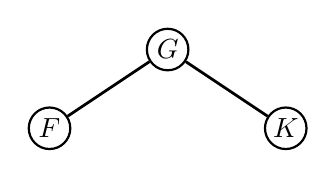
\begin{tikzpicture}[>=latex, thick, inner sep=0pt, scale=0.5]
			\node[circle, draw=black, minimum size=15pt](G) at (0,0) {$G$};
			\node[circle, draw=black, minimum size=15pt](F) at (-3,-2) {$F$};
			\node[circle, draw=black, minimum size=15pt](K) at (3,-2) {$K$};
			
			\draw[-, line width=1pt](G) edge (F);
			\draw[-, line width=1pt](G) edge (K);
		\end{tikzpicture}
	\label{Result after step 1 tree}
	\end{figure} \par
\end{minipage}
\vspace*{15mm}



\underline{Step 3.} \par
Now, we split in $y-$direction. Hence, we sort $x_{above}$ and $x_{below}$ in $y-direction$ and split each of them into two new lists $y_{above_1}$, $y_{above_2}$ for the left and right upper part analogously for the part below. Then we get: \par
\vspace*{-3mm}
\begin{equation}
\begin{aligned}
y_{above_1} & \coloneqq [A,D,E] \hspace*{18mm} && y_{above_2} \coloneqq [B,C] \\[3pt]
y_{below_1} & \coloneqq [H,I,M] && y_{below_2} \coloneqq [J,L]
\end{aligned}
\end{equation} \par
For $y_{above_2}$ and $y_{below_2}$ we have to use $R4$ to calculate the middle elements. Let $M$ be a function which calculates the middle elements for a list, by the given rules, then we get: \par
\begin{equation}
\begin{aligned}
M(y_{above_1}) & = D \hspace*{18mm} && M(y_{above_2}) = C \\[3pt]
M(y_{below_1}) & = I && M(y_{below_2}) = L
\end{aligned}
\end{equation}
Updating the tree and the lines in the plane yields to: \par
\vspace*{-5mm}
\begin{minipage}[t]{0.48\textwidth}
\begin{figure}[H]
\centering
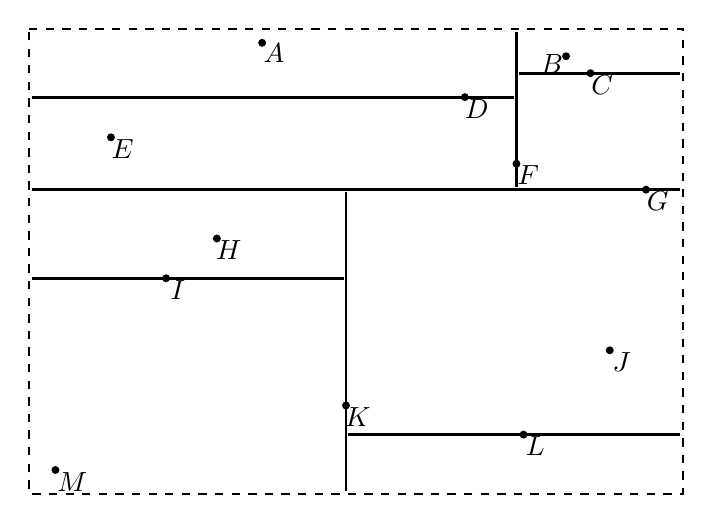
\begin{tikzpicture}[>=latex, thick, inner sep=0pt, scale=0.5]
	
	
	\draw[black,thick,dashed] (0,0) -- (16.6,0) -- (16.6,-11.8) -- (0,-11.8) -- (0,0);
	
	\node[circle, fill, draw=black, minimum size=2pt](a) at (5.92,-0.35) {};
	\node[circle, fill, draw=black, minimum size=2pt](b) at (13.64,-0.69) {};
	\node[circle, fill, draw=black, minimum size=2pt](c) at (14.26,-1.12) {};
	\node[circle, fill, draw=black, minimum size=2pt](d) at (11.07,-1.73) {};
	\node[circle, fill, draw=black, minimum size=2pt](e) at (2.08,-2.75) {};
	\node[circle, fill, draw=black, minimum size=2pt](f) at (12.38,-3.42) {};
	\node[circle, fill, draw=black, minimum size=2pt](g) at (15.67,-4.08) {};
	\node[circle, fill, draw=black, minimum size=2pt](h) at (4.77,-5.32) {};
	\node[circle, fill, draw=black, minimum size=2pt](i) at (3.48,-6.33) {};
	\node[circle, fill, draw=black, minimum size=2pt](j) at (14.75,-8.16) {};
	\node[circle, fill, draw=black, minimum size=2pt](k) at (8.05,-9.56) {};
	\node[circle, fill, draw=black, minimum size=2pt](l) at (12.56,-10.3) {};
	\node[circle, fill, draw=black, minimum size=2pt](m) at (0.67,-11.2) {};
		
		
	\node[](A) at (6.22,-0.6) {$A$};
	\node[](B) at (13.28,-0.9) {$B$};
	\node[](C) at (14.56,-1.42) {$C$};
	\node[](D) at (11.37,-2.03) {$D$};
	\node[](E) at (2.38,-3.05) {$E$};
	\node[](F) at (12.68,-3.72) {$F$};
	\node[](G) at (15.97,-4.38) {$G$};
	\node[](H) at (5.07,-5.62) {$H$};
	\node[](I) at (3.78,-6.63) {$I$};
	\node[](J) at (15.05,-8.46) {$J$};
	\node[](K) at (8.35,-9.86) {$K$};
	\node[](L) at (12.86,-10.6) {$L$};
	\node[](M) at (1.1,-11.5) {$M$};

	\node[](a_start) at (5.92,0) {};
	\node[](a_ende) at (5.92,-1.73) {};
	
	\node[](b_start) at (13.64,0) {};
	\node[](b_ende) at (13.64,-1.12) {};

	\node[](c_start) at (12.38,-1.12) {};
	\node[](c_ende) at (16.6,-1.12) {};
	
	\node[](d_start) at (0.0,-1.73) {};
	\node[](d_ende) at (12.38,-1.73) {};
	
	\node[](e_start) at (2.08,-1.73) {};
	\node[](e_ende) at (2.08,-4.08) {};
	
	\node[](f_start) at (12.38,0) {};
	\node[](f_ende) at (12.38,-4.08) {};
	
	\node[](g_start) at (0.0,-4.08) {};
	\node[](g_ende) at (16.6,-4.08) {};
	
	\node[](h_start) at (4.77,-4.08) {};
	\node[](h_ende) at (4.77,-6.33) {};
	
	\node[](i_start) at (0.0,-6.33) {};
	\node[](i_ende) at (8.05,-6.33) {};
	
	\node[](j_start) at (14.75,-4.08) {};
	\node[](j_ende) at (14.75,-10.3) {};
	
	\node[](k_start) at (8.05,-4.08) {};
	\node[](k_ende) at (8.05,-11.8) {};

	\node[](l_start) at (8.05,-10.3) {};
	\node[](l_ende) at (16.6,-10.3) {};

	\node[](m_start) at (0.67,-6.33) {};
	\node[](m_ende) at (0.67,-11.8) {};
	
	% vertikale Linen			
	\draw[-, line width=1pt](f_start) edge (f_ende);				
	\draw[-, line width=1pt](k_start) edge (k_ende);	



	% horizontale Linen
	\draw[-, line width=1pt](c_start) edge (c_ende);	
	\draw[-, line width=1pt](d_start) edge (d_ende);		
	\draw[-, line width=1pt](g_start) edge (g_ende);			
	\draw[-, line width=1pt](i_start) edge (i_ende);			
	\draw[-, line width=1pt](l_start) edge (l_ende);			
\end{tikzpicture}
\label{Result after step 1}
\end{figure} \par
\end{minipage} \hspace*{5mm}
\begin{minipage}[t]{0.45\textwidth}
	\begin{figure}[H]
		\centering
		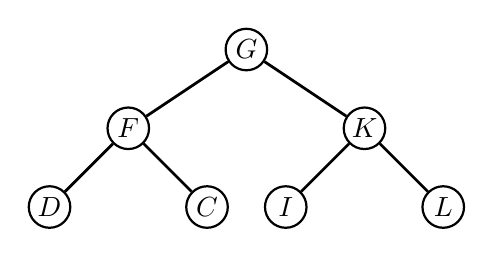
\begin{tikzpicture}[>=latex, thick, inner sep=0pt, scale=0.5]
			\node[circle, draw=black, minimum size=15pt](G) at (0,0) {$G$};
			
			\node[circle, draw=black, minimum size=15pt](F) at (-3,-2) {$F$};
			\node[circle, draw=black, minimum size=15pt](K) at (3,-2) {$K$};

			\node[circle, draw=black, minimum size=15pt](D) at (-5,-4) {$D$};
			\node[circle, draw=black, minimum size=15pt](C) at (-1,-4) {$C$};
			\node[circle, draw=black, minimum size=15pt](I) at (1,-4) {$I$};
			\node[circle, draw=black, minimum size=15pt](L) at (5,-4) {$L$};
			
			\draw[-, line width=1pt](G) edge (F);
			\draw[-, line width=1pt](G) edge (K);
			
			\draw[-, line width=1pt](F) edge (D);
			\draw[-, line width=1pt](F) edge (C);
			
			\draw[-, line width=1pt](K) edge (I);
			\draw[-, line width=1pt](K) edge (L);
		\end{tikzpicture}
	\label{Result after step 1 tree}
	\end{figure} \par
\end{minipage}
\newpage


\underline{Step 4.} \par
Now, we are splitting in $x-$direction. Since each remaining list only contains at least one element, we are done after insert those elements in the $kD-$tree. Again, by using $R3$ for inserting the new child nodes, we get: \par
\begin{figure}[H]
	\centering
	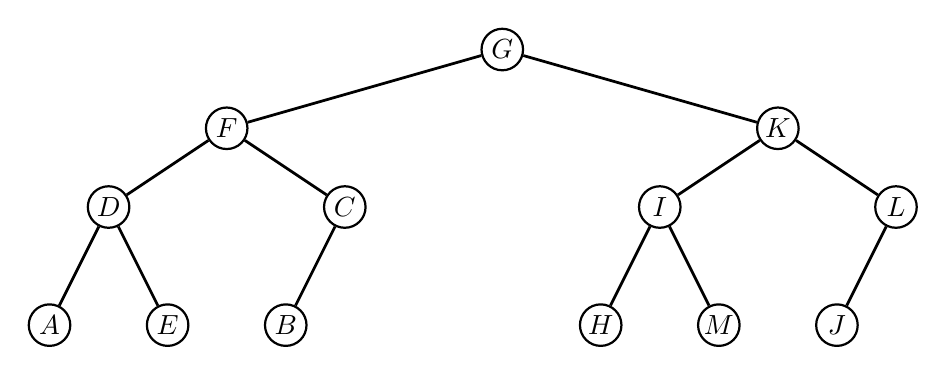
\begin{tikzpicture}[>=latex, thick, inner sep=0pt, scale=0.5]
		\node[circle, draw=black, minimum size=15pt](G) at (0,0) {$G$};
		
		\node[circle, draw=black, minimum size=15pt](F) at (-7,-2) {$F$};
		\node[circle, draw=black, minimum size=15pt](K) at (7,-2) {$K$};

		\node[circle, draw=black, minimum size=15pt](D) at (-10,-4) {$D$};
		\node[circle, draw=black, minimum size=15pt](C) at (-4,-4) {$C$};
		\node[circle, draw=black, minimum size=15pt](I) at (4,-4) {$I$};
		\node[circle, draw=black, minimum size=15pt](L) at (10,-4) {$L$};

		\node[circle, draw=black, minimum size=15pt](A) at (-11.5,-7) {$A$};
		\node[circle, draw=black, minimum size=15pt](E) at (-8.5,-7) {$E$};
		\node[circle, draw=black, minimum size=15pt](B) at (-5.5,-7) {$B$};
		\node[circle, draw=black, minimum size=15pt](H) at (2.5,-7) {$H$};
		\node[circle, draw=black, minimum size=15pt](M) at (5.5,-7) {$M$};
		\node[circle, draw=black, minimum size=15pt](J) at (8.5,-7) {$J$};

		
		\draw[-, line width=1pt](G) edge (F);
		\draw[-, line width=1pt](G) edge (K);
		
		\draw[-, line width=1pt](F) edge (D);
		\draw[-, line width=1pt](F) edge (C);
		
		\draw[-, line width=1pt](K) edge (I);
		\draw[-, line width=1pt](K) edge (L);

		\draw[-, line width=1pt](D) edge (A);
		\draw[-, line width=1pt](D) edge (E);
		\draw[-, line width=1pt](C) edge (B);
		\draw[-, line width=1pt](I) edge (H);
		\draw[-, line width=1pt](I) edge (M);
		\draw[-, line width=1pt](L) edge (J);
	\end{tikzpicture}
\label{Result after step 1 tree}
\end{figure} \par
\vspace*{20mm}


\begin{figure}[H]
\renewcommand{\thefigure}{2.4.2}
\centering
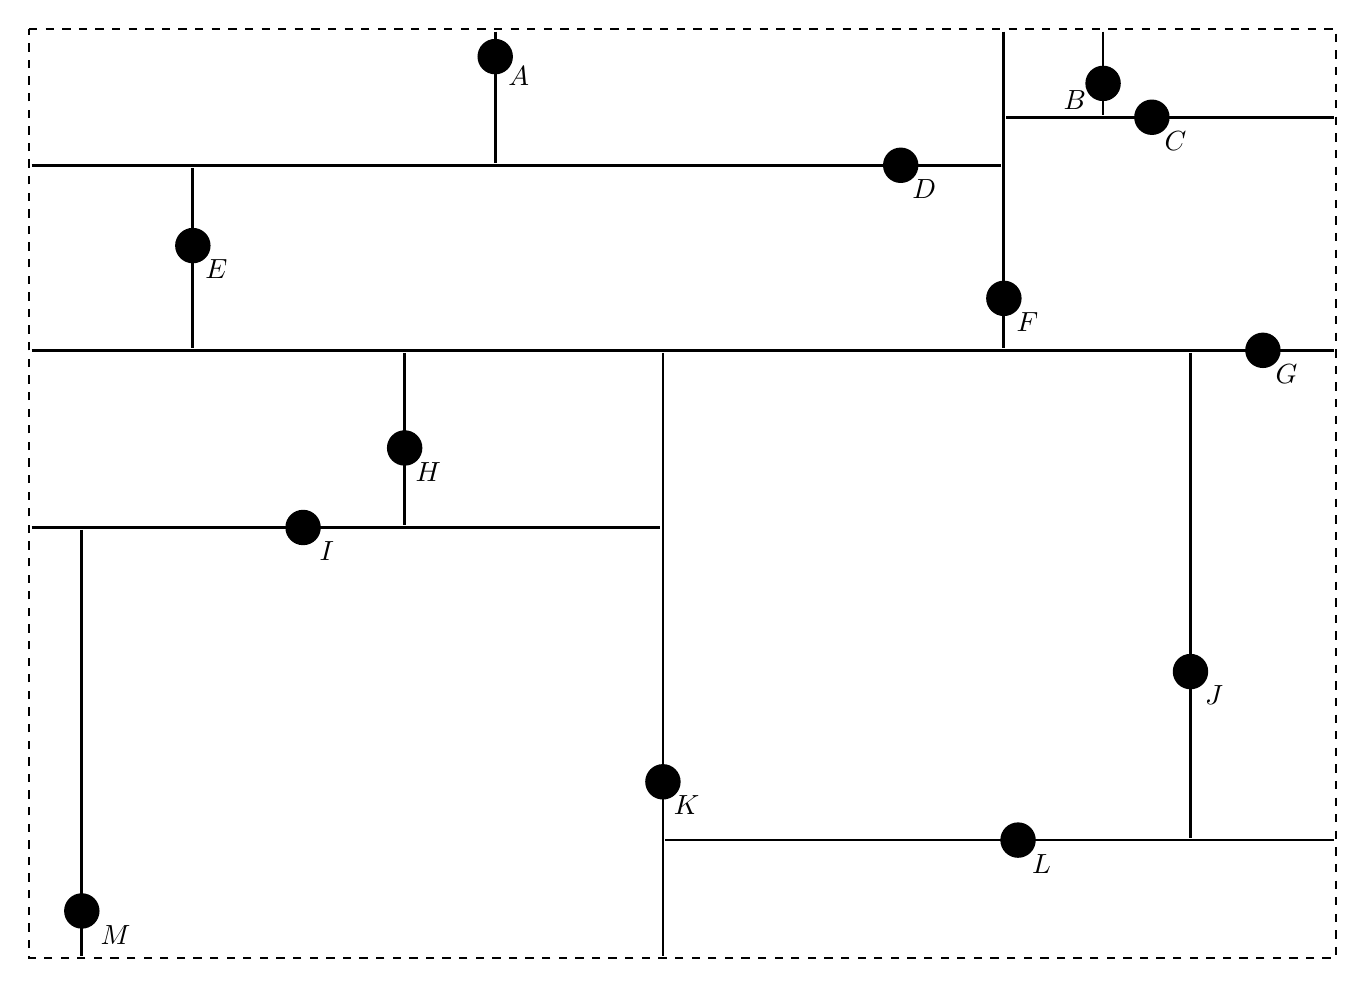
\begin{tikzpicture}[>=latex, thick, inner sep=0pt, scale=1]
	
	
	\draw[black,thick,dashed] (0,0) -- (16.6,0) -- (16.6,-11.8) -- (0,-11.8) -- (0,0);
	
	\node[circle, fill, draw=black, minimum size=12pt](a) at (5.92,-0.35) {};
	\node[circle, fill, draw=black, minimum size=12pt](b) at (13.64,-0.69) {};
	\node[circle, fill, draw=black, minimum size=12pt](c) at (14.26,-1.12) {};
	\node[circle, fill, draw=black, minimum size=12pt](d) at (11.07,-1.73) {};
	\node[circle, fill, draw=black, minimum size=12pt](e) at (2.08,-2.75) {};
	\node[circle, fill, draw=black, minimum size=12pt](f) at (12.38,-3.42) {};
	\node[circle, fill, draw=black, minimum size=12pt](g) at (15.67,-4.08) {};
	\node[circle, fill, draw=black, minimum size=12pt](h) at (4.77,-5.32) {};
	\node[circle, fill, draw=black, minimum size=12pt](i) at (3.48,-6.33) {};
	\node[circle, fill, draw=black, minimum size=12pt](j) at (14.75,-8.16) {};
	\node[circle, fill, draw=black, minimum size=12pt](k) at (8.05,-9.56) {};
	\node[circle, fill, draw=black, minimum size=12pt](l) at (12.56,-10.3) {};
	\node[circle, fill, draw=black, minimum size=12pt](m) at (0.67,-11.2) {};
		
		
	\node[](A) at (6.22,-0.6) {$A$};
	\node[](B) at (13.28,-0.9) {$B$};
	\node[](C) at (14.56,-1.42) {$C$};
	\node[](D) at (11.37,-2.03) {$D$};
	\node[](E) at (2.38,-3.05) {$E$};
	\node[](F) at (12.68,-3.72) {$F$};
	\node[](G) at (15.97,-4.38) {$G$};
	\node[](H) at (5.07,-5.62) {$H$};
	\node[](I) at (3.78,-6.63) {$I$};
	\node[](J) at (15.05,-8.46) {$J$};
	\node[](K) at (8.35,-9.86) {$K$};
	\node[](L) at (12.86,-10.6) {$L$};
	\node[](M) at (1.1,-11.5) {$M$};

	\node[](a_start) at (5.92,0) {};
	\node[](a_ende) at (5.92,-1.73) {};
	
	\node[](b_start) at (13.64,0) {};
	\node[](b_ende) at (13.64,-1.12) {};

	\node[](c_start) at (12.38,-1.12) {};
	\node[](c_ende) at (16.6,-1.12) {};
	
	\node[](d_start) at (0.0,-1.73) {};
	\node[](d_ende) at (12.38,-1.73) {};
	
	\node[](e_start) at (2.08,-1.73) {};
	\node[](e_ende) at (2.08,-4.08) {};
	
	\node[](f_start) at (12.38,0) {};
	\node[](f_ende) at (12.38,-4.08) {};
	
	\node[](g_start) at (0.0,-4.08) {};
	\node[](g_ende) at (16.6,-4.08) {};
	
	\node[](h_start) at (4.77,-4.08) {};
	\node[](h_ende) at (4.77,-6.33) {};
	
	\node[](i_start) at (0.0,-6.33) {};
	\node[](i_ende) at (8.05,-6.33) {};
	
	\node[](j_start) at (14.75,-4.08) {};
	\node[](j_ende) at (14.75,-10.3) {};
	
	\node[](k_start) at (8.05,-4.08) {};
	\node[](k_ende) at (8.05,-11.8) {};

	\node[](l_start) at (8.05,-10.3) {};
	\node[](l_ende) at (16.6,-10.3) {};

	\node[](m_start) at (0.67,-6.33) {};
	\node[](m_ende) at (0.67,-11.8) {};
	
	% vertikale Linen
	\draw[-, line width=1pt](a_start) edge (a_ende);	
	\draw[-, line width=1pt](b_start) edge (b_ende);		
	\draw[-, line width=1pt](e_start) edge (e_ende);			
	\draw[-, line width=1pt](f_start) edge (f_ende);			
	\draw[-, line width=1pt](h_start) edge (h_ende);					
	\draw[-, line width=1pt](j_start) edge (j_ende);	
	\draw[-, line width=1pt](k_start) edge (k_ende);	
	\draw[-, line width=1pt](m_start) edge (m_ende);


	% horizontale Linen
	\draw[-, line width=1pt](c_start) edge (c_ende);	
	\draw[-, line width=1pt](d_start) edge (d_ende);		
	\draw[-, line width=1pt](g_start) edge (g_ende);			
	\draw[-, line width=1pt](i_start) edge (i_ende);			
	\draw[-, line width=1pt](l_start) edge (l_ende);

\end{tikzpicture}
\end{figure} \par
\vspace*{2mm}
\vspace*{15mm}




\newpage

\section*{\large Exercise 3 (Range Search in a kD-tree) {\normalsize \hfill (5 points)}}


\section*{\large Exercise 4 (Nearest Neighbor Search in a kD Tree) {\normalsize \hfill (4 points)}}

\end{document}

